\documentclass[1p]{elsarticle_modified}
%\bibliographystyle{elsarticle-num}

%\usepackage[colorlinks]{hyperref}
%\usepackage{abbrmath_seonhwa} %\Abb, \Ascr, \Acal ,\Abf, \Afrak
\usepackage{amsfonts}
\usepackage{amssymb}
\usepackage{amsmath}
\usepackage{amsthm}
\usepackage{scalefnt}
\usepackage{amsbsy}
\usepackage{kotex}
\usepackage{caption}
\usepackage{subfig}
\usepackage{color}
\usepackage{graphicx}
\usepackage{xcolor} %% white, black, red, green, blue, cyan, magenta, yellow
\usepackage{float}
\usepackage{setspace}
\usepackage{hyperref}

\usepackage{tikz}
\usetikzlibrary{arrows}

\usepackage{multirow}
\usepackage{array} % fixed length table
\usepackage{hhline}

%%%%%%%%%%%%%%%%%%%%%
\makeatletter
\renewcommand*\env@matrix[1][\arraystretch]{%
	\edef\arraystretch{#1}%
	\hskip -\arraycolsep
	\let\@ifnextchar\new@ifnextchar
	\array{*\c@MaxMatrixCols c}}
\makeatother %https://tex.stackexchange.com/questions/14071/how-can-i-increase-the-line-spacing-in-a-matrix
%%%%%%%%%%%%%%%

\usepackage[normalem]{ulem}

\newcommand{\msout}[1]{\ifmmode\text{\sout{\ensuremath{#1}}}\else\sout{#1}\fi}
%SOURCE: \msout is \stkout macro in https://tex.stackexchange.com/questions/20609/strikeout-in-math-mode

\newcommand{\cancel}[1]{
	\ifmmode
	{\color{red}\msout{#1}}
	\else
	{\color{red}\sout{#1}}
	\fi
}

\newcommand{\add}[1]{
	{\color{blue}\uwave{#1}}
}

\newcommand{\replace}[2]{
	\ifmmode
	{\color{red}\msout{#1}}{\color{blue}\uwave{#2}}
	\else
	{\color{red}\sout{#1}}{\color{blue}\uwave{#2}}
	\fi
}

\newcommand{\Sol}{\mathcal{S}} %segment
\newcommand{\D}{D} %diagram
\newcommand{\A}{\mathcal{A}} %arc


%%%%%%%%%%%%%%%%%%%%%%%%%%%%%5 test

\def\sl{\operatorname{\textup{SL}}(2,\Cbb)}
\def\psl{\operatorname{\textup{PSL}}(2,\Cbb)}
\def\quan{\mkern 1mu \triangleright \mkern 1mu}

\theoremstyle{definition}
\newtheorem{thm}{Theorem}[section]
\newtheorem{prop}[thm]{Proposition}
\newtheorem{lem}[thm]{Lemma}
\newtheorem{ques}[thm]{Question}
\newtheorem{cor}[thm]{Corollary}
\newtheorem{defn}[thm]{Definition}
\newtheorem{exam}[thm]{Example}
\newtheorem{rmk}[thm]{Remark}
\newtheorem{alg}[thm]{Algorithm}

\newcommand{\I}{\sqrt{-1}}
\begin{document}

%\begin{frontmatter}
%
%\title{Boundary parabolic representations of knots up to 8 crossings}
%
%%% Group authors per affiliation:
%\author{Yunhi Cho} 
%\address{Department of Mathematics, University of Seoul, Seoul, Korea}
%\ead{yhcho@uos.ac.kr}
%
%
%\author{Seonhwa Kim} %\fnref{s_kim}}
%\address{Center for Geometry and Physics, Institute for Basic Science, Pohang, 37673, Korea}
%\ead{ryeona17@ibs.re.kr}
%
%\author{Hyuk Kim}
%\address{Department of Mathematical Sciences, Seoul National University, Seoul 08826, Korea}
%\ead{hyukkim@snu.ac.kr}
%
%\author{Seokbeom Yoon}
%\address{Department of Mathematical Sciences, Seoul National University, Seoul, 08826,  Korea}
%\ead{sbyoon15@snu.ac.kr}
%
%\begin{abstract}
%We find all boundary parabolic representation of knots up to 8 crossings.
%
%\end{abstract}
%\begin{keyword}
%    \MSC[2010] 57M25 
%\end{keyword}
%
%\end{frontmatter}

%\linenumbers
%\tableofcontents
%
\newcommand\colored[1]{\textcolor{white}{\rule[-0.35ex]{0.8em}{1.4ex}}\kern-0.8em\color{red} #1}%
%\newcommand\colored[1]{\textcolor{white}{ #1}\kern-2.17ex	\textcolor{white}{ #1}\kern-1.81ex	\textcolor{white}{ #1}\kern-2.15ex\color{red}#1	}

{\Large $\underline{12a_{0152}~(K12a_{0152})}$}

\setlength{\tabcolsep}{10pt}
\renewcommand{\arraystretch}{1.6}
\vspace{1cm}\begin{tabular}{m{100pt}>{\centering\arraybackslash}m{274pt}}
\multirow{5}{120pt}{
	\centering
	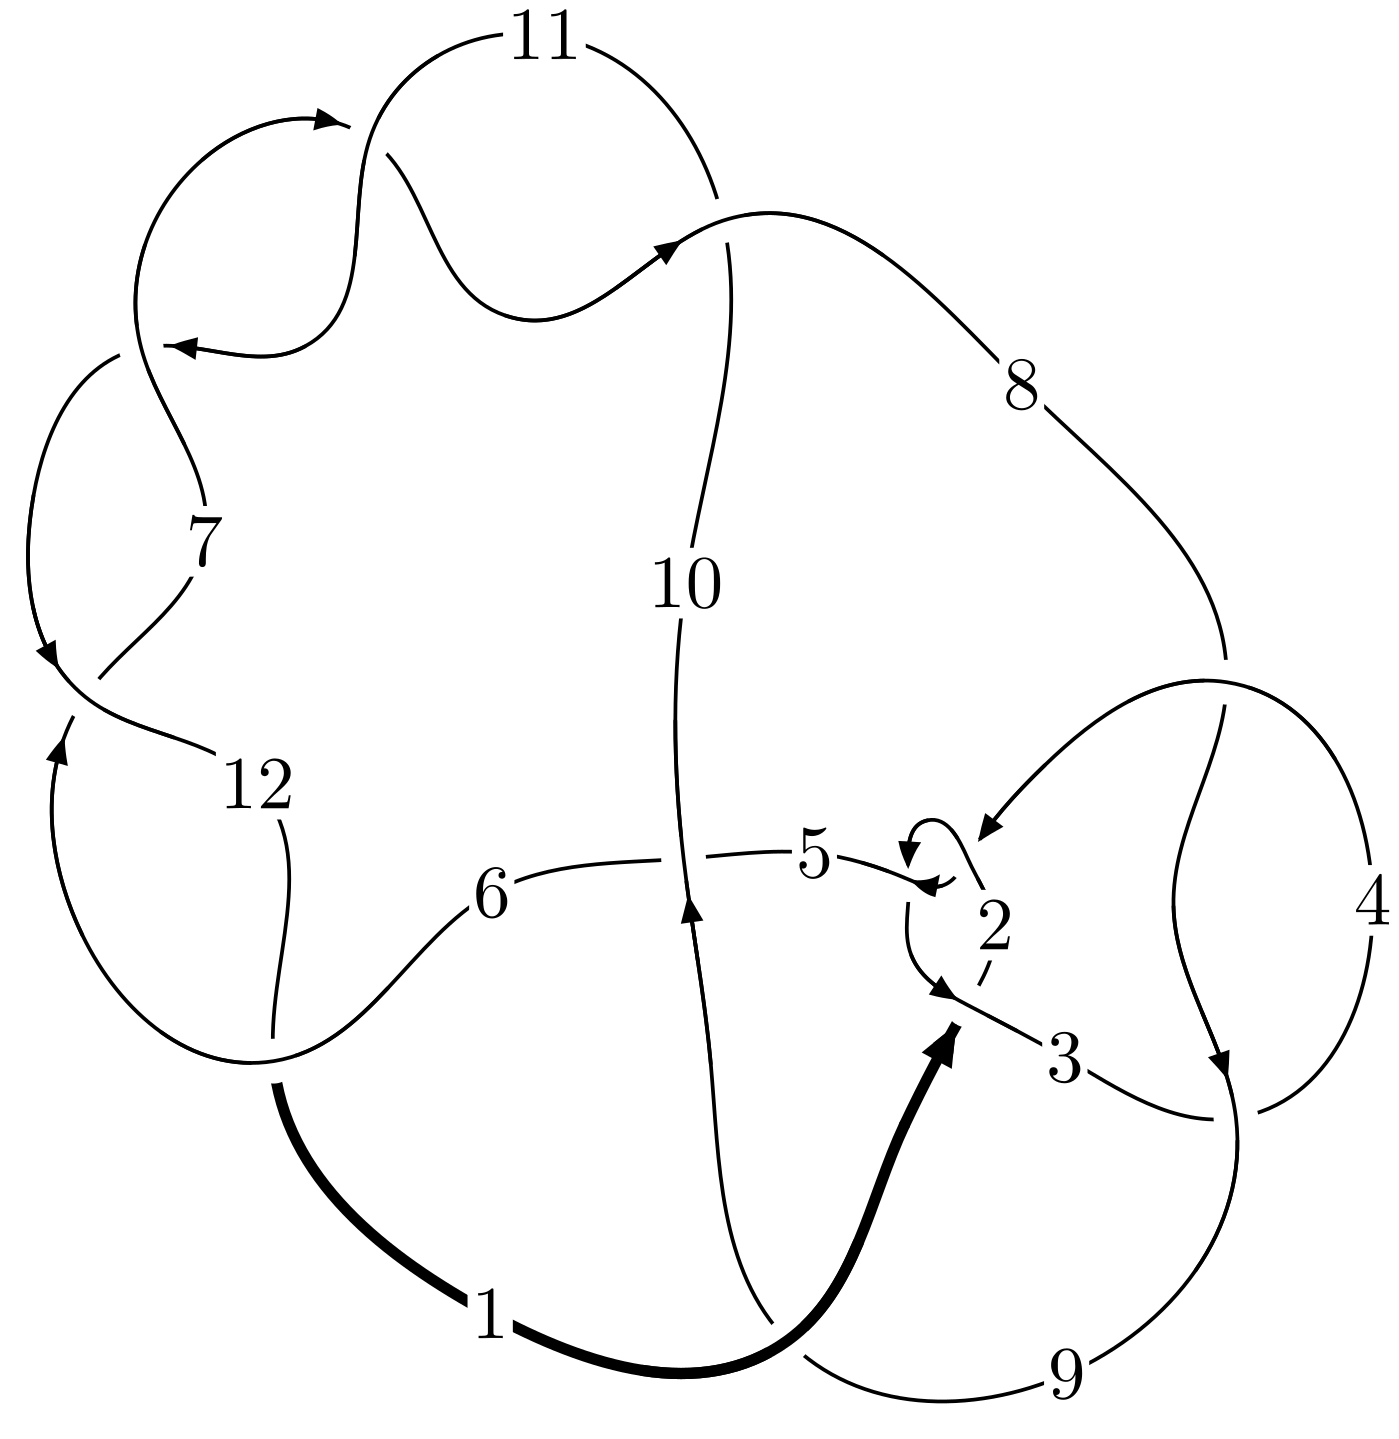
\includegraphics[width=112pt]{../../../GIT/diagram.site/Diagrams/png/953_12a_0152.png}\\
\ \ \ A knot diagram\footnotemark}&
\allowdisplaybreaks
\textbf{Linearized knot diagam} \\
\cline{2-2}
 &
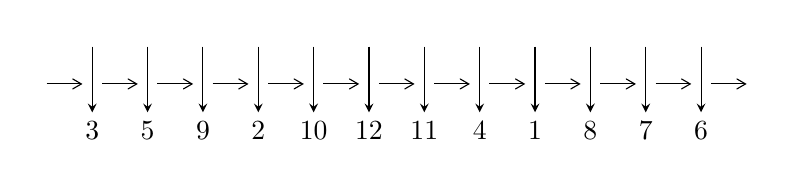
\begin{tikzpicture}[x=20pt, y=17pt]
	% nodes
	\node (C0) at (0, 0) {};
	\node (C1) at (1, 0) {};
	\node (C1U) at (1, +1) {};
	\node (C1D) at (1, -1) {3};

	\node (C2) at (2, 0) {};
	\node (C2U) at (2, +1) {};
	\node (C2D) at (2, -1) {5};

	\node (C3) at (3, 0) {};
	\node (C3U) at (3, +1) {};
	\node (C3D) at (3, -1) {9};

	\node (C4) at (4, 0) {};
	\node (C4U) at (4, +1) {};
	\node (C4D) at (4, -1) {2};

	\node (C5) at (5, 0) {};
	\node (C5U) at (5, +1) {};
	\node (C5D) at (5, -1) {10};

	\node (C6) at (6, 0) {};
	\node (C6U) at (6, +1) {};
	\node (C6D) at (6, -1) {12};

	\node (C7) at (7, 0) {};
	\node (C7U) at (7, +1) {};
	\node (C7D) at (7, -1) {11};

	\node (C8) at (8, 0) {};
	\node (C8U) at (8, +1) {};
	\node (C8D) at (8, -1) {4};

	\node (C9) at (9, 0) {};
	\node (C9U) at (9, +1) {};
	\node (C9D) at (9, -1) {1};

	\node (C10) at (10, 0) {};
	\node (C10U) at (10, +1) {};
	\node (C10D) at (10, -1) {8};

	\node (C11) at (11, 0) {};
	\node (C11U) at (11, +1) {};
	\node (C11D) at (11, -1) {7};

	\node (C12) at (12, 0) {};
	\node (C12U) at (12, +1) {};
	\node (C12D) at (12, -1) {6};
	\node (C13) at (13, 0) {};

	% arrows
	\draw[->,>={angle 60}]
	(C0) edge (C1) (C1) edge (C2) (C2) edge (C3) (C3) edge (C4) (C4) edge (C5) (C5) edge (C6) (C6) edge (C7) (C7) edge (C8) (C8) edge (C9) (C9) edge (C10) (C10) edge (C11) (C11) edge (C12) (C12) edge (C13) ;	\draw[->,>=stealth]
	(C1U) edge (C1D) (C2U) edge (C2D) (C3U) edge (C3D) (C4U) edge (C4D) (C5U) edge (C5D) (C6U) edge (C6D) (C7U) edge (C7D) (C8U) edge (C8D) (C9U) edge (C9D) (C10U) edge (C10D) (C11U) edge (C11D) (C12U) edge (C12D) ;
	\end{tikzpicture} \\
\hhline{~~} \\& 
\textbf{Solving Sequence} \\ \cline{2-2} 
 &
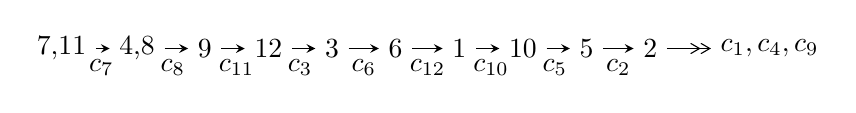
\begin{tikzpicture}[x=23pt, y=7pt]
	% node
	\node (A0) at (-1/8, 0) {7,11};
	\node (A1) at (17/16, 0) {4,8};
	\node (A2) at (17/8, 0) {9};
	\node (A3) at (25/8, 0) {12};
	\node (A4) at (33/8, 0) {3};
	\node (A5) at (41/8, 0) {6};
	\node (A6) at (49/8, 0) {1};
	\node (A7) at (57/8, 0) {10};
	\node (A8) at (65/8, 0) {5};
	\node (A9) at (73/8, 0) {2};
	\node (C1) at (1/2, -1) {$c_{7}$};
	\node (C2) at (13/8, -1) {$c_{8}$};
	\node (C3) at (21/8, -1) {$c_{11}$};
	\node (C4) at (29/8, -1) {$c_{3}$};
	\node (C5) at (37/8, -1) {$c_{6}$};
	\node (C6) at (45/8, -1) {$c_{12}$};
	\node (C7) at (53/8, -1) {$c_{10}$};
	\node (C8) at (61/8, -1) {$c_{5}$};
	\node (C9) at (69/8, -1) {$c_{2}$};
	\node (A10) at (11, 0) {$c_{1},c_{4},c_{9}$};

	% edge
	\draw[->,>=stealth]	
	(A0) edge (A1) (A1) edge (A2) (A2) edge (A3) (A3) edge (A4) (A4) edge (A5) (A5) edge (A6) (A6) edge (A7) (A7) edge (A8) (A8) edge (A9) ;
	\draw[->>,>={angle 60}]	
	(A9) edge (A10);
\end{tikzpicture} \\ 

\end{tabular} \\

\footnotetext{
The image of knot diagram is generated by the software ``\textbf{Draw programme}" developed by Andrew Bartholomew(\url{http://www.layer8.co.uk/maths/draw/index.htm\#Running-draw}), where we modified some parts for our purpose(\url{https://github.com/CATsTAILs/LinksPainter}).
}\phantom \\ \newline 
\centering \textbf{Ideals for irreducible components\footnotemark of $X_{\text{par}}$} 
 
\begin{align*}
I^u_{1}&=\langle 
2 u^{59}+3 u^{58}+\cdots+b-1,\;u^{60}+39 u^{58}+\cdots+a+1,\;u^{61}+2 u^{60}+\cdots- u-1\rangle \\
I^u_{2}&=\langle 
- u^3+u^2+b-2 u+1,\;u^4+3 u^2+a+1,\;u^5- u^4+4 u^3-3 u^2+3 u-1\rangle \\
\\
\end{align*}
\raggedright * 2 irreducible components of $\dim_{\mathbb{C}}=0$, with total 66 representations.\\
\footnotetext{All coefficients of polynomials are rational numbers. But the coefficients are sometimes approximated in decimal forms when there is not enough margin.}
\newpage
\renewcommand{\arraystretch}{1}
\centering \section*{I. $I^u_{1}= \langle 2 u^{59}+3 u^{58}+\cdots+b-1,\;u^{60}+39 u^{58}+\cdots+a+1,\;u^{61}+2 u^{60}+\cdots- u-1 \rangle$}
\flushleft \textbf{(i) Arc colorings}\\
\begin{tabular}{m{7pt} m{180pt} m{7pt} m{180pt} }
\flushright $a_{7}=$&$\begin{pmatrix}1\\0\end{pmatrix}$ \\
\flushright $a_{11}=$&$\begin{pmatrix}0\\u\end{pmatrix}$ \\
\flushright $a_{4}=$&$\begin{pmatrix}- u^{60}-39 u^{58}+\cdots- u^2-1\\-2 u^{59}-3 u^{58}+\cdots+2 u+1\end{pmatrix}$ \\
\flushright $a_{8}=$&$\begin{pmatrix}1\\u^2\end{pmatrix}$ \\
\flushright $a_{9}=$&$\begin{pmatrix}u^9+6 u^7+11 u^5+6 u^3+u\\- u^9-5 u^7-7 u^5-2 u^3+u\end{pmatrix}$ \\
\flushright $a_{12}=$&$\begin{pmatrix}- u\\u\end{pmatrix}$ \\
\flushright $a_{3}=$&$\begin{pmatrix}- u^{60}-2 u^{59}+\cdots-3 u^3- u^2\\- u^{58}-2 u^{57}+\cdots+u+1\end{pmatrix}$ \\
\flushright $a_{6}=$&$\begin{pmatrix}u^2+1\\- u^2\end{pmatrix}$ \\
\flushright $a_{1}=$&$\begin{pmatrix}- u^3-2 u\\u^3+u\end{pmatrix}$ \\
\flushright $a_{10}=$&$\begin{pmatrix}u\\u^3+u\end{pmatrix}$ \\
\flushright $a_{5}=$&$\begin{pmatrix}- u^6-3 u^4+1\\- u^8-4 u^6-4 u^4-2 u^2\end{pmatrix}$ \\
\flushright $a_{2}=$&$\begin{pmatrix}- u^{60}- u^{59}+\cdots+2 u^3-2 u^2\\- u^{59}-2 u^{58}+\cdots+2 u+1\end{pmatrix}$\\&\end{tabular}
\flushleft \textbf{(ii) Obstruction class $= -1$}\\~\\
\flushleft \textbf{(iii) Cusp Shapes $= u^{60}+2 u^{59}+\cdots-13 u-14$}\\~\\
\newpage\renewcommand{\arraystretch}{1}
\flushleft \textbf{(iv) u-Polynomials at the component}\newline \\
\begin{tabular}{m{50pt}|m{274pt}}
Crossings & \hspace{64pt}u-Polynomials at each crossing \\
\hline $$\begin{aligned}c_{1}\end{aligned}$$&$\begin{aligned}
&u^{61}+28 u^{60}+\cdots+25 u+1
\end{aligned}$\\
\hline $$\begin{aligned}c_{2},c_{4}\end{aligned}$$&$\begin{aligned}
&u^{61}-6 u^{60}+\cdots+u+1
\end{aligned}$\\
\hline $$\begin{aligned}c_{3},c_{8}\end{aligned}$$&$\begin{aligned}
&u^{61}- u^{60}+\cdots+32 u+32
\end{aligned}$\\
\hline $$\begin{aligned}c_{5}\end{aligned}$$&$\begin{aligned}
&u^{61}-2 u^{60}+\cdots+3487 u+389
\end{aligned}$\\
\hline $$\begin{aligned}c_{6},c_{7},c_{10}\\c_{11},c_{12}\end{aligned}$$&$\begin{aligned}
&u^{61}-2 u^{60}+\cdots- u+1
\end{aligned}$\\
\hline $$\begin{aligned}c_{9}\end{aligned}$$&$\begin{aligned}
&u^{61}+8 u^{60}+\cdots+6443 u+1751
\end{aligned}$\\
\hline
\end{tabular}\\~\\
\newpage\renewcommand{\arraystretch}{1}
\flushleft \textbf{(v) Riley Polynomials at the component}\newline \\
\begin{tabular}{m{50pt}|m{274pt}}
Crossings & \hspace{64pt}Riley Polynomials at each crossing \\
\hline $$\begin{aligned}c_{1}\end{aligned}$$&$\begin{aligned}
&y^{61}+16 y^{60}+\cdots+1049 y-1
\end{aligned}$\\
\hline $$\begin{aligned}c_{2},c_{4}\end{aligned}$$&$\begin{aligned}
&y^{61}-28 y^{60}+\cdots+25 y-1
\end{aligned}$\\
\hline $$\begin{aligned}c_{3},c_{8}\end{aligned}$$&$\begin{aligned}
&y^{61}+33 y^{60}+\cdots-9728 y-1024
\end{aligned}$\\
\hline $$\begin{aligned}c_{5}\end{aligned}$$&$\begin{aligned}
&y^{61}+16 y^{60}+\cdots+1506015 y-151321
\end{aligned}$\\
\hline $$\begin{aligned}c_{6},c_{7},c_{10}\\c_{11},c_{12}\end{aligned}$$&$\begin{aligned}
&y^{61}+80 y^{60}+\cdots+7 y-1
\end{aligned}$\\
\hline $$\begin{aligned}c_{9}\end{aligned}$$&$\begin{aligned}
&y^{61}+28 y^{60}+\cdots-9774541 y-3066001
\end{aligned}$\\
\hline
\end{tabular}\\~\\
\newpage\flushleft \textbf{(vi) Complex Volumes and Cusp Shapes}
$$\begin{array}{c|c|c}  
\text{Solutions to }I^u_{1}& \I (\text{vol} + \sqrt{-1}CS) & \text{Cusp shape}\\
 \hline 
\begin{aligned}
u &= -0.254354 + 0.981103 I \\
a &= -1.25198 - 2.54671 I \\
b &= \phantom{-}0.07492 + 2.00861 I\end{aligned}
 & \phantom{-}1.22942 + 3.29969 I & \phantom{-0.000000 } 0 \\ \hline\begin{aligned}
u &= -0.254354 - 0.981103 I \\
a &= -1.25198 + 2.54671 I \\
b &= \phantom{-}0.07492 - 2.00861 I\end{aligned}
 & \phantom{-}1.22942 - 3.29969 I & \phantom{-0.000000 } 0 \\ \hline\begin{aligned}
u &= \phantom{-}0.211321 + 1.001770 I \\
a &= -0.322034 - 0.875785 I \\
b &= -0.289419 + 0.657547 I\end{aligned}
 & \phantom{-}3.12919 - 1.33617 I & \phantom{-0.000000 } 0 \\ \hline\begin{aligned}
u &= \phantom{-}0.211321 - 1.001770 I \\
a &= -0.322034 + 0.875785 I \\
b &= -0.289419 - 0.657547 I\end{aligned}
 & \phantom{-}3.12919 + 1.33617 I & \phantom{-0.000000 } 0 \\ \hline\begin{aligned}
u &= \phantom{-}0.281128 + 0.997371 I \\
a &= \phantom{-}0.582713 + 0.789402 I \\
b &= \phantom{-}0.070322 - 0.761861 I\end{aligned}
 & \phantom{-}2.34136 - 5.73880 I & \phantom{-0.000000 } 0 \\ \hline\begin{aligned}
u &= \phantom{-}0.281128 - 0.997371 I \\
a &= \phantom{-}0.582713 - 0.789402 I \\
b &= \phantom{-}0.070322 + 0.761861 I\end{aligned}
 & \phantom{-}2.34136 + 5.73880 I & \phantom{-0.000000 } 0 \\ \hline\begin{aligned}
u &= -0.328410 + 1.012920 I \\
a &= -1.51065 - 2.03863 I \\
b &= \phantom{-}0.68097 + 1.62757 I\end{aligned}
 & \phantom{-}5.15125 + 11.89640 I & \phantom{-0.000000 } 0 \\ \hline\begin{aligned}
u &= -0.328410 - 1.012920 I \\
a &= -1.51065 + 2.03863 I \\
b &= \phantom{-}0.68097 - 1.62757 I\end{aligned}
 & \phantom{-}5.15125 - 11.89640 I & \phantom{-0.000000 } 0 \\ \hline\begin{aligned}
u &= -0.302074 + 1.025430 I \\
a &= \phantom{-}1.38727 + 2.07338 I \\
b &= -0.49004 - 1.57864 I\end{aligned}
 & \phantom{-}7.28412 + 6.15559 I & \phantom{-0.000000 } 0 \\ \hline\begin{aligned}
u &= -0.302074 - 1.025430 I \\
a &= \phantom{-}1.38727 - 2.07338 I \\
b &= -0.49004 + 1.57864 I\end{aligned}
 & \phantom{-}7.28412 - 6.15559 I & \phantom{-0.000000 } 0\\
 \hline 
 \end{array}$$\newpage$$\begin{array}{c|c|c}  
\text{Solutions to }I^u_{1}& \I (\text{vol} + \sqrt{-1}CS) & \text{Cusp shape}\\
 \hline 
\begin{aligned}
u &= \phantom{-}0.316983 + 0.866277 I \\
a &= \phantom{-}0.824553 + 0.132321 I \\
b &= -0.397869 - 0.455885 I\end{aligned}
 & \phantom{-}1.00389 - 1.16184 I & \phantom{-0.000000 } 0 \\ \hline\begin{aligned}
u &= \phantom{-}0.316983 - 0.866277 I \\
a &= \phantom{-}0.824553 - 0.132321 I \\
b &= -0.397869 + 0.455885 I\end{aligned}
 & \phantom{-}1.00389 + 1.16184 I & \phantom{-0.000000 } 0 \\ \hline\begin{aligned}
u &= -0.207432 + 1.073920 I \\
a &= \phantom{-}0.85102 + 1.88063 I \\
b &= \phantom{-}0.092713 - 1.158660 I\end{aligned}
 & \phantom{-}8.38349 + 1.96602 I & \phantom{-0.000000 } 0 \\ \hline\begin{aligned}
u &= -0.207432 - 1.073920 I \\
a &= \phantom{-}0.85102 - 1.88063 I \\
b &= \phantom{-}0.092713 + 1.158660 I\end{aligned}
 & \phantom{-}8.38349 - 1.96602 I & \phantom{-0.000000 } 0 \\ \hline\begin{aligned}
u &= -0.156803 + 1.097010 I \\
a &= -0.65117 - 1.69342 I \\
b &= -0.278390 + 0.945645 I\end{aligned}
 & \phantom{-}7.08755 - 3.73090 I & \phantom{-0.000000 } 0 \\ \hline\begin{aligned}
u &= -0.156803 - 1.097010 I \\
a &= -0.65117 + 1.69342 I \\
b &= -0.278390 - 0.945645 I\end{aligned}
 & \phantom{-}7.08755 + 3.73090 I & \phantom{-0.000000 } 0 \\ \hline\begin{aligned}
u &= \phantom{-}0.148119 + 0.845043 I \\
a &= \phantom{-}0.414383 - 0.713810 I \\
b &= -0.575491 + 0.156747 I\end{aligned}
 & \phantom{-}1.88176 - 1.60682 I & -5.29446 + 5.04055 I \\ \hline\begin{aligned}
u &= \phantom{-}0.148119 - 0.845043 I \\
a &= \phantom{-}0.414383 + 0.713810 I \\
b &= -0.575491 - 0.156747 I\end{aligned}
 & \phantom{-}1.88176 + 1.60682 I & -5.29446 - 5.04055 I \\ \hline\begin{aligned}
u &= \phantom{-}0.325121 + 0.738493 I \\
a &= -1.089280 + 0.346297 I \\
b &= \phantom{-}0.705617 + 0.283188 I\end{aligned}
 & \phantom{-}0.29625 - 4.76842 I & -9.08610 + 8.21702 I \\ \hline\begin{aligned}
u &= \phantom{-}0.325121 - 0.738493 I \\
a &= -1.089280 - 0.346297 I \\
b &= \phantom{-}0.705617 - 0.283188 I\end{aligned}
 & \phantom{-}0.29625 + 4.76842 I & -9.08610 - 8.21702 I\\
 \hline 
 \end{array}$$\newpage$$\begin{array}{c|c|c}  
\text{Solutions to }I^u_{1}& \I (\text{vol} + \sqrt{-1}CS) & \text{Cusp shape}\\
 \hline 
\begin{aligned}
u &= -0.092397 + 0.693687 I \\
a &= -1.029970 + 0.913793 I \\
b &= \phantom{-}1.174630 + 0.233112 I\end{aligned}
 & -0.987120 + 0.988516 I & -11.84015 - 0.12287 I \\ \hline\begin{aligned}
u &= -0.092397 - 0.693687 I \\
a &= -1.029970 - 0.913793 I \\
b &= \phantom{-}1.174630 - 0.233112 I\end{aligned}
 & -0.987120 - 0.988516 I & -11.84015 + 0.12287 I \\ \hline\begin{aligned}
u &= -0.429667 + 0.466787 I \\
a &= \phantom{-}0.300862 - 0.006110 I \\
b &= \phantom{-}0.537163 + 1.081280 I\end{aligned}
 & \phantom{-}2.11665 - 5.58640 I & -9.13002 + 1.98520 I \\ \hline\begin{aligned}
u &= -0.429667 - 0.466787 I \\
a &= \phantom{-}0.300862 + 0.006110 I \\
b &= \phantom{-}0.537163 - 1.081280 I\end{aligned}
 & \phantom{-}2.11665 + 5.58640 I & -9.13002 - 1.98520 I \\ \hline\begin{aligned}
u &= -0.556702 + 0.224542 I \\
a &= \phantom{-}2.03671 + 0.31639 I \\
b &= -0.005895 + 0.791176 I\end{aligned}
 & \phantom{-}1.32668 + 8.88717 I & -11.5386 - 8.5026 I \\ \hline\begin{aligned}
u &= -0.556702 - 0.224542 I \\
a &= \phantom{-}2.03671 - 0.31639 I \\
b &= -0.005895 - 0.791176 I\end{aligned}
 & \phantom{-}1.32668 - 8.88717 I & -11.5386 + 8.5026 I \\ \hline\begin{aligned}
u &= -0.437350 + 0.391378 I \\
a &= -0.666219 - 0.260171 I \\
b &= -0.393377 - 0.987812 I\end{aligned}
 & \phantom{-}3.80352 - 0.17614 I & -6.56300 - 3.19514 I \\ \hline\begin{aligned}
u &= -0.437350 - 0.391378 I \\
a &= -0.666219 + 0.260171 I \\
b &= -0.393377 + 0.987812 I\end{aligned}
 & \phantom{-}3.80352 + 0.17614 I & -6.56300 + 3.19514 I \\ \hline\begin{aligned}
u &= -0.523029 + 0.253421 I \\
a &= -1.74252 - 0.41441 I \\
b &= -0.088899 - 0.841462 I\end{aligned}
 & \phantom{-}3.32476 + 3.34552 I & -8.30796 - 4.53572 I \\ \hline\begin{aligned}
u &= -0.523029 - 0.253421 I \\
a &= -1.74252 + 0.41441 I \\
b &= -0.088899 + 0.841462 I\end{aligned}
 & \phantom{-}3.32476 - 3.34552 I & -8.30796 + 4.53572 I\\
 \hline 
 \end{array}$$\newpage$$\begin{array}{c|c|c}  
\text{Solutions to }I^u_{1}& \I (\text{vol} + \sqrt{-1}CS) & \text{Cusp shape}\\
 \hline 
\begin{aligned}
u &= \phantom{-}0.544484 + 0.051126 I \\
a &= \phantom{-}0.271290 - 1.260450 I \\
b &= -0.152520 + 0.534984 I\end{aligned}
 & -1.77296 + 1.77637 I & -13.44810 - 3.42636 I \\ \hline\begin{aligned}
u &= \phantom{-}0.544484 - 0.051126 I \\
a &= \phantom{-}0.271290 + 1.260450 I \\
b &= -0.152520 - 0.534984 I\end{aligned}
 & -1.77296 - 1.77637 I & -13.44810 + 3.42636 I \\ \hline\begin{aligned}
u &= \phantom{-}0.479319 + 0.211089 I \\
a &= \phantom{-}0.97175 - 1.13377 I \\
b &= -0.539313 + 0.342045 I\end{aligned}
 & -1.38873 - 3.13575 I & -13.6527 + 6.6645 I \\ \hline\begin{aligned}
u &= \phantom{-}0.479319 - 0.211089 I \\
a &= \phantom{-}0.97175 + 1.13377 I \\
b &= -0.539313 - 0.342045 I\end{aligned}
 & -1.38873 + 3.13575 I & -13.6527 - 6.6645 I \\ \hline\begin{aligned}
u &= -0.425241 + 0.171006 I \\
a &= \phantom{-}1.80164 + 1.52641 I \\
b &= \phantom{-}0.240942 + 0.694488 I\end{aligned}
 & -2.33602 + 0.95454 I & -12.3987 - 7.0289 I \\ \hline\begin{aligned}
u &= -0.425241 - 0.171006 I \\
a &= \phantom{-}1.80164 - 1.52641 I \\
b &= \phantom{-}0.240942 - 0.694488 I\end{aligned}
 & -2.33602 - 0.95454 I & -12.3987 + 7.0289 I \\ \hline\begin{aligned}
u &= \phantom{-}0.307712 + 0.317136 I \\
a &= -1.21859 + 0.96164 I \\
b &= \phantom{-}0.621069 - 0.032600 I\end{aligned}
 & -0.798120 + 0.509659 I & -11.36907 + 1.74616 I \\ \hline\begin{aligned}
u &= \phantom{-}0.307712 - 0.317136 I \\
a &= -1.21859 - 0.96164 I \\
b &= \phantom{-}0.621069 + 0.032600 I\end{aligned}
 & -0.798120 - 0.509659 I & -11.36907 - 1.74616 I \\ \hline\begin{aligned}
u &= \phantom{-}0.04390 + 1.64371 I \\
a &= \phantom{-}0.471528 - 0.589481 I \\
b &= -1.69900 + 0.69117 I\end{aligned}
 & \phantom{-}8.54157 - 5.92897 I & \phantom{-0.000000 } 0 \\ \hline\begin{aligned}
u &= \phantom{-}0.04390 - 1.64371 I \\
a &= \phantom{-}0.471528 + 0.589481 I \\
b &= -1.69900 - 0.69117 I\end{aligned}
 & \phantom{-}8.54157 + 5.92897 I & \phantom{-0.000000 } 0\\
 \hline 
 \end{array}$$\newpage$$\begin{array}{c|c|c}  
\text{Solutions to }I^u_{1}& \I (\text{vol} + \sqrt{-1}CS) & \text{Cusp shape}\\
 \hline 
\begin{aligned}
u &= -0.00808 + 1.66823 I \\
a &= \phantom{-}0.636613 - 0.961433 I \\
b &= -2.50286 + 1.98917 I\end{aligned}
 & \phantom{-}7.54962 + 1.22321 I & \phantom{-0.000000 } 0 \\ \hline\begin{aligned}
u &= -0.00808 - 1.66823 I \\
a &= \phantom{-}0.636613 + 0.961433 I \\
b &= -2.50286 - 1.98917 I\end{aligned}
 & \phantom{-}7.54962 - 1.22321 I & \phantom{-0.000000 } 0 \\ \hline\begin{aligned}
u &= \phantom{-}0.07133 + 1.68137 I \\
a &= -0.481555 + 0.218553 I \\
b &= \phantom{-}1.133360 + 0.000284 I\end{aligned}
 & \phantom{-}9.95685 - 2.59158 I & \phantom{-0.000000 } 0 \\ \hline\begin{aligned}
u &= \phantom{-}0.07133 - 1.68137 I \\
a &= -0.481555 - 0.218553 I \\
b &= \phantom{-}1.133360 - 0.000284 I\end{aligned}
 & \phantom{-}9.95685 + 2.59158 I & \phantom{-0.000000 } 0 \\ \hline\begin{aligned}
u &= \phantom{-}0.02693 + 1.68333 I \\
a &= -0.182151 + 0.761285 I \\
b &= \phantom{-}1.04861 - 1.56495 I\end{aligned}
 & \phantom{-}10.86580 - 2.21377 I & \phantom{-0.000000 } 0 \\ \hline\begin{aligned}
u &= \phantom{-}0.02693 - 1.68333 I \\
a &= -0.182151 - 0.761285 I \\
b &= \phantom{-}1.04861 + 1.56495 I\end{aligned}
 & \phantom{-}10.86580 + 2.21377 I & \phantom{-0.000000 } 0 \\ \hline\begin{aligned}
u &= \phantom{-}0.316056\phantom{ +0.000000I} \\
a &= -1.09435\phantom{ +0.000000I} \\
b &= \phantom{-}0.309110\phantom{ +0.000000I}\end{aligned}
 & -0.608532\phantom{ +0.000000I} & -16.3260\phantom{ +0.000000I} \\ \hline\begin{aligned}
u &= -0.06576 + 1.71571 I \\
a &= \phantom{-}0.82473 + 2.57511 I \\
b &= -2.07010 - 6.76803 I\end{aligned}
 & \phantom{-}10.82330 + 4.58248 I & \phantom{-0.000000 } 0 \\ \hline\begin{aligned}
u &= -0.06576 - 1.71571 I \\
a &= \phantom{-}0.82473 - 2.57511 I \\
b &= -2.07010 + 6.76803 I\end{aligned}
 & \phantom{-}10.82330 - 4.58248 I & \phantom{-0.000000 } 0 \\ \hline\begin{aligned}
u &= \phantom{-}0.07278 + 1.71903 I \\
a &= -0.769346 - 0.337131 I \\
b &= \phantom{-}1.25059 + 1.17834 I\end{aligned}
 & \phantom{-}11.99390 - 7.16364 I & \phantom{-0.000000 } 0\\
 \hline 
 \end{array}$$\newpage$$\begin{array}{c|c|c}  
\text{Solutions to }I^u_{1}& \I (\text{vol} + \sqrt{-1}CS) & \text{Cusp shape}\\
 \hline 
\begin{aligned}
u &= \phantom{-}0.07278 - 1.71903 I \\
a &= -0.769346 + 0.337131 I \\
b &= \phantom{-}1.25059 - 1.17834 I\end{aligned}
 & \phantom{-}11.99390 + 7.16364 I & \phantom{-0.000000 } 0 \\ \hline\begin{aligned}
u &= \phantom{-}0.05627 + 1.72019 I \\
a &= \phantom{-}0.607773 + 0.556302 I \\
b &= -0.85094 - 1.51707 I\end{aligned}
 & \phantom{-}12.83490 - 2.42911 I & \phantom{-0.000000 } 0 \\ \hline\begin{aligned}
u &= \phantom{-}0.05627 - 1.72019 I \\
a &= \phantom{-}0.607773 - 0.556302 I \\
b &= -0.85094 + 1.51707 I\end{aligned}
 & \phantom{-}12.83490 + 2.42911 I & \phantom{-0.000000 } 0 \\ \hline\begin{aligned}
u &= -0.08659 + 1.72253 I \\
a &= \phantom{-}0.88576 + 2.17643 I \\
b &= -2.64835 - 5.43557 I\end{aligned}
 & \phantom{-}14.8480 + 13.5808 I & \phantom{-0.000000 } 0 \\ \hline\begin{aligned}
u &= -0.08659 - 1.72253 I \\
a &= \phantom{-}0.88576 - 2.17643 I \\
b &= -2.64835 + 5.43557 I\end{aligned}
 & \phantom{-}14.8480 - 13.5808 I & \phantom{-0.000000 } 0 \\ \hline\begin{aligned}
u &= -0.07895 + 1.72628 I \\
a &= -0.83698 - 2.26090 I \\
b &= \phantom{-}2.34895 + 5.64277 I\end{aligned}
 & \phantom{-}17.0651 + 7.7083 I & \phantom{-0.000000 } 0 \\ \hline\begin{aligned}
u &= -0.07895 - 1.72628 I \\
a &= -0.83698 + 2.26090 I \\
b &= \phantom{-}2.34895 - 5.64277 I\end{aligned}
 & \phantom{-}17.0651 - 7.7083 I & \phantom{-0.000000 } 0 \\ \hline\begin{aligned}
u &= -0.05183 + 1.73689 I \\
a &= -0.57601 - 2.21329 I \\
b &= \phantom{-}1.15538 + 5.39428 I\end{aligned}
 & \phantom{-}18.4431 + 3.0304 I & \phantom{-0.000000 } 0 \\ \hline\begin{aligned}
u &= -0.05183 - 1.73689 I \\
a &= -0.57601 + 2.21329 I \\
b &= \phantom{-}1.15538 - 5.39428 I\end{aligned}
 & \phantom{-}18.4431 - 3.0304 I & \phantom{-0.000000 } 0 \\ \hline\begin{aligned}
u &= -0.03876 + 1.73935 I \\
a &= \phantom{-}0.50704 + 2.06226 I \\
b &= -0.80734 - 4.96112 I\end{aligned}
 & \phantom{-}17.2479 - 2.9269 I & \phantom{-0.000000 } 0\\
 \hline 
 \end{array}$$\newpage$$\begin{array}{c|c|c}  
\text{Solutions to }I^u_{1}& \I (\text{vol} + \sqrt{-1}CS) & \text{Cusp shape}\\
 \hline 
\begin{aligned}
u &= -0.03876 - 1.73935 I \\
a &= \phantom{-}0.50704 - 2.06226 I \\
b &= -0.80734 + 4.96112 I\end{aligned}
 & \phantom{-}17.2479 + 2.9269 I & \phantom{-0.000000 } 0\\
 \hline 
 \end{array}$$\newpage\newpage\renewcommand{\arraystretch}{1}
\centering \section*{II. $I^u_{2}= \langle - u^3+u^2+b-2 u+1,\;u^4+3 u^2+a+1,\;u^5- u^4+4 u^3-3 u^2+3 u-1 \rangle$}
\flushleft \textbf{(i) Arc colorings}\\
\begin{tabular}{m{7pt} m{180pt} m{7pt} m{180pt} }
\flushright $a_{7}=$&$\begin{pmatrix}1\\0\end{pmatrix}$ \\
\flushright $a_{11}=$&$\begin{pmatrix}0\\u\end{pmatrix}$ \\
\flushright $a_{4}=$&$\begin{pmatrix}- u^4-3 u^2-1\\u^3- u^2+2 u-1\end{pmatrix}$ \\
\flushright $a_{8}=$&$\begin{pmatrix}1\\u^2\end{pmatrix}$ \\
\flushright $a_{9}=$&$\begin{pmatrix}1\\u^2\end{pmatrix}$ \\
\flushright $a_{12}=$&$\begin{pmatrix}- u\\u\end{pmatrix}$ \\
\flushright $a_{3}=$&$\begin{pmatrix}- u^4-3 u^2-1\\u^3- u^2+2 u-1\end{pmatrix}$ \\
\flushright $a_{6}=$&$\begin{pmatrix}u^2+1\\- u^2\end{pmatrix}$ \\
\flushright $a_{1}=$&$\begin{pmatrix}- u^3-2 u\\u^3+u\end{pmatrix}$ \\
\flushright $a_{10}=$&$\begin{pmatrix}u\\u^3+u\end{pmatrix}$ \\
\flushright $a_{5}=$&$\begin{pmatrix}u^3+2 u\\- u^3- u\end{pmatrix}$ \\
\flushright $a_{2}=$&$\begin{pmatrix}- u^4- u^3-3 u^2-2 u-1\\2 u^3- u^2+3 u-1\end{pmatrix}$\\&\end{tabular}
\flushleft \textbf{(ii) Obstruction class $= 1$}\\~\\
\flushleft \textbf{(iii) Cusp Shapes $= -3 u^4+3 u^3-12 u^2+10 u-19$}\\~\\
\newpage\renewcommand{\arraystretch}{1}
\flushleft \textbf{(iv) u-Polynomials at the component}\newline \\
\begin{tabular}{m{50pt}|m{274pt}}
Crossings & \hspace{64pt}u-Polynomials at each crossing \\
\hline $$\begin{aligned}c_{1},c_{2}\end{aligned}$$&$\begin{aligned}
&(u-1)^5
\end{aligned}$\\
\hline $$\begin{aligned}c_{3},c_{8}\end{aligned}$$&$\begin{aligned}
&u^5
\end{aligned}$\\
\hline $$\begin{aligned}c_{4}\end{aligned}$$&$\begin{aligned}
&(u+1)^5
\end{aligned}$\\
\hline $$\begin{aligned}c_{5},c_{9}\end{aligned}$$&$\begin{aligned}
&u^5- u^4+u^2+u-1
\end{aligned}$\\
\hline $$\begin{aligned}c_{6},c_{7}\end{aligned}$$&$\begin{aligned}
&u^5- u^4+4 u^3-3 u^2+3 u-1
\end{aligned}$\\
\hline $$\begin{aligned}c_{10},c_{11},c_{12}\end{aligned}$$&$\begin{aligned}
&u^5+u^4+4 u^3+3 u^2+3 u+1
\end{aligned}$\\
\hline
\end{tabular}\\~\\
\newpage\renewcommand{\arraystretch}{1}
\flushleft \textbf{(v) Riley Polynomials at the component}\newline \\
\begin{tabular}{m{50pt}|m{274pt}}
Crossings & \hspace{64pt}Riley Polynomials at each crossing \\
\hline $$\begin{aligned}c_{1},c_{2},c_{4}\end{aligned}$$&$\begin{aligned}
&(y-1)^5
\end{aligned}$\\
\hline $$\begin{aligned}c_{3},c_{8}\end{aligned}$$&$\begin{aligned}
&y^5
\end{aligned}$\\
\hline $$\begin{aligned}c_{5},c_{9}\end{aligned}$$&$\begin{aligned}
&y^5- y^4+4 y^3-3 y^2+3 y-1
\end{aligned}$\\
\hline $$\begin{aligned}c_{6},c_{7},c_{10}\\c_{11},c_{12}\end{aligned}$$&$\begin{aligned}
&y^5+7 y^4+16 y^3+13 y^2+3 y-1
\end{aligned}$\\
\hline
\end{tabular}\\~\\
\newpage\flushleft \textbf{(vi) Complex Volumes and Cusp Shapes}
$$\begin{array}{c|c|c}  
\text{Solutions to }I^u_{2}& \I (\text{vol} + \sqrt{-1}CS) & \text{Cusp shape}\\
 \hline 
\begin{aligned}
u &= \phantom{-}0.233677 + 0.885557 I \\
a &= \phantom{-}0.827780 - 0.637683 I \\
b &= -0.340036 + 0.807849 I\end{aligned}
 & \phantom{-}0.17487 - 2.21397 I & -10.60206 + 4.05273 I \\ \hline\begin{aligned}
u &= \phantom{-}0.233677 - 0.885557 I \\
a &= \phantom{-}0.827780 + 0.637683 I \\
b &= -0.340036 - 0.807849 I\end{aligned}
 & \phantom{-}0.17487 + 2.21397 I & -10.60206 - 4.05273 I \\ \hline\begin{aligned}
u &= \phantom{-}0.416284\phantom{ +0.000000I} \\
a &= -1.54991\phantom{ +0.000000I} \\
b &= -0.268586\phantom{ +0.000000I}\end{aligned}
 & -2.52712\phantom{ +0.000000I} & -16.7900\phantom{ +0.000000I} \\ \hline\begin{aligned}
u &= \phantom{-}0.05818 + 1.69128 I \\
a &= -0.552827 + 0.534136 I \\
b &= \phantom{-}1.47433 - 1.63485 I\end{aligned}
 & \phantom{-}9.31336 - 3.33174 I & -10.00277 + 3.46299 I \\ \hline\begin{aligned}
u &= \phantom{-}0.05818 - 1.69128 I \\
a &= -0.552827 - 0.534136 I \\
b &= \phantom{-}1.47433 + 1.63485 I\end{aligned}
 & \phantom{-}9.31336 + 3.33174 I & -10.00277 - 3.46299 I\\
 \hline 
 \end{array}$$\newpage
\newpage\renewcommand{\arraystretch}{1}
\centering \section*{ III. u-Polynomials}
\begin{tabular}{m{50pt}|m{274pt}}
Crossings & \hspace{64pt}u-Polynomials at each crossing \\
\hline $$\begin{aligned}c_{1}\end{aligned}$$&$\begin{aligned}
&((u-1)^5)(u^{61}+28 u^{60}+\cdots+25 u+1)
\end{aligned}$\\
\hline $$\begin{aligned}c_{2}\end{aligned}$$&$\begin{aligned}
&((u-1)^5)(u^{61}-6 u^{60}+\cdots+u+1)
\end{aligned}$\\
\hline $$\begin{aligned}c_{3},c_{8}\end{aligned}$$&$\begin{aligned}
&u^5(u^{61}- u^{60}+\cdots+32 u+32)
\end{aligned}$\\
\hline $$\begin{aligned}c_{4}\end{aligned}$$&$\begin{aligned}
&((u+1)^5)(u^{61}-6 u^{60}+\cdots+u+1)
\end{aligned}$\\
\hline $$\begin{aligned}c_{5}\end{aligned}$$&$\begin{aligned}
&(u^5- u^4+u^2+u-1)(u^{61}-2 u^{60}+\cdots+3487 u+389)
\end{aligned}$\\
\hline $$\begin{aligned}c_{6},c_{7}\end{aligned}$$&$\begin{aligned}
&(u^5- u^4+4 u^3-3 u^2+3 u-1)(u^{61}-2 u^{60}+\cdots- u+1)
\end{aligned}$\\
\hline $$\begin{aligned}c_{9}\end{aligned}$$&$\begin{aligned}
&(u^5- u^4+u^2+u-1)(u^{61}+8 u^{60}+\cdots+6443 u+1751)
\end{aligned}$\\
\hline $$\begin{aligned}c_{10},c_{11},c_{12}\end{aligned}$$&$\begin{aligned}
&(u^5+u^4+4 u^3+3 u^2+3 u+1)(u^{61}-2 u^{60}+\cdots- u+1)
\end{aligned}$\\
\hline
\end{tabular}\newpage\renewcommand{\arraystretch}{1}
\centering \section*{ IV. Riley Polynomials}
\begin{tabular}{m{50pt}|m{274pt}}
Crossings & \hspace{64pt}Riley Polynomials at each crossing \\
\hline $$\begin{aligned}c_{1}\end{aligned}$$&$\begin{aligned}
&((y-1)^5)(y^{61}+16 y^{60}+\cdots+1049 y-1)
\end{aligned}$\\
\hline $$\begin{aligned}c_{2},c_{4}\end{aligned}$$&$\begin{aligned}
&((y-1)^5)(y^{61}-28 y^{60}+\cdots+25 y-1)
\end{aligned}$\\
\hline $$\begin{aligned}c_{3},c_{8}\end{aligned}$$&$\begin{aligned}
&y^5(y^{61}+33 y^{60}+\cdots-9728 y-1024)
\end{aligned}$\\
\hline $$\begin{aligned}c_{5}\end{aligned}$$&$\begin{aligned}
&(y^5- y^4+4 y^3-3 y^2+3 y-1)\\
&\cdot(y^{61}+16 y^{60}+\cdots+1506015 y-151321)
\end{aligned}$\\
\hline $$\begin{aligned}c_{6},c_{7},c_{10}\\c_{11},c_{12}\end{aligned}$$&$\begin{aligned}
&(y^5+7 y^4+16 y^3+13 y^2+3 y-1)(y^{61}+80 y^{60}+\cdots+7 y-1)
\end{aligned}$\\
\hline $$\begin{aligned}c_{9}\end{aligned}$$&$\begin{aligned}
&(y^5- y^4+4 y^3-3 y^2+3 y-1)\\
&\cdot(y^{61}+28 y^{60}+\cdots-9774541 y-3066001)
\end{aligned}$\\
\hline
\end{tabular}
\vskip 2pc
\end{document}